%%%%%%%%%%%%%%%%%%%%%%%%%%%%% Define Exam %%%%%%%%%%%%%%%%%%%%%%%%%%%%%%%%%%
\documentclass[addpoints]{exam}
%%%%%%%%%%%%%%%%%%%%%%%%%%%%%%%%%%%%%%%%%%%%%%%%%%%%%%%%%%%%%%%%%%%%%%%%%%%%%%%

%%%%%%%%%%%%%%%%%%%%%%%%%%%%% Using Packages %%%%%%%%%%%%%%%%%%%%%%%%%%%%%%%%%%
\usepackage[utf8]{inputenc}
\usepackage{float, geometry, graphicx, color, xcolor, colortbl}
\usepackage{amsmath, amssymb, amsthm, amsfonts, geometry, venndiagram, tikz, comment}
\usepackage{wrapfig, parskip, tabularx}
\usepackage{colortbl}
\usepackage{listings, mdframed, lipsum, psfrag, empheq, verbatim, subfig, hyperref, cite}
\usepackage{bookmark, booktabs, titlesec, subfig, pdfpages, lastpage, pagerange}
\usepackage{pythonhighlight}
\usepackage{upgreek, pifont}
\usepackage{multirow}
\usepackage{multicol}
\usepackage{times}
\usepackage{setspace}


% Expectation symbol
\DeclareMathOperator*{\E}{\mathbb{E}}

%%%%%%%%%%%%%%%%%%%%%%%%%%%%%%%%%%%%%%%%%%%%%%%%%%%%%%%%%%%%%%%%%%%%%%%%%%%%%%%
\definecolor{codebackground}{rgb}{0.95,0.95,0.95}
\definecolor{codegray}{rgb}{0.5,0.5,0.5}
\definecolor{codepurple}{rgb}{0.58,0,0.82}
\definecolor{codeblue}{rgb}{0.13,0.29,0.53}
\definecolor{ocre}{RGB}{243,102,25}
\definecolor{mygray}{RGB}{243,243,244}
\definecolor{deepGreen}{RGB}{26,111,0}
\definecolor{shallowGreen}{RGB}{235,255,255}
\definecolor{deepBlue}{RGB}{61,124,222}
\definecolor{shallowBlue}{RGB}{235,249,255}
\definecolor{softgray}{rgb}{0.95, 0.95, 0.95}



%%%%%%%%%%%%%%%%%%%%%%%%%%%%% Header and Footer %%%%%%%%%%%%%%%%%%%%%%%%%%%%%%%%%%
\pagestyle{headandfoot}
\runningheadrule
\runningfootrule
\runningheader{Reinforcement Learning}{Assignment 01}{CS/CE 353/368}
\runningfooter{}{Page \thepage\ of \numpages}{}
\firstpageheader{}{}{}
%%%%%%%%%%%%%%%%%%%%%%%%%%%%%%%%%%%%%%%%%%%%%%%%%%%%%%%%%%%%%%%%%%%%%%%%%%%%%%%

% Other Settings
% \boxedpoints
\printanswers
\qformat{}  %Comment this to number questions, uncomment this to not number questions

\newcommand\union\cup
\newcommand\inter\cap

%%%%%%%%%%%%%%%%%%%%%%%%%%%%%%% Title & Author %%%%%%%%%%%%%%%%%%%%%%%%%%%%%%%%
\title{{\huge \textbf{Reinforcement Learning CS/CE 353/368}} 

\vspace*{1mm}
{\LARGE \textbf{Assignment 01}}

{
\includegraphics[width=0.45\textwidth]{logo.png}} \\}

\author{Ali Muhammad - aa07190}
\date{}

% \pgfplotsset{compat=1.18}

%%%%%%%%%%%%%%%%%%%%%%%%%%%%%%%%%%%%%%%%%%%%%%%%%%%%%%%%%%%%%%%%%%%%%%%%%%%%%%%

\begin{document}
\maketitle

{\small \begin{center}
    \gradetable[h]
  \end{center}}

\newpage
\begin{questions}
\question[50]
\subsection*{Q1 - [50 points] - Environment Setup}

\begin{solution}
\begin{enumerate}
    \item[(a)] \textbf{[05 points]} 

    $ |\mathcal{S}| $ denotes the total number of possible states in the grid, which can be represented as $ m \times n \times |\{ N, E, S, W \}| $ where the set $ \{ N, E, S, W \} $ denotes the four possible directions (North, East, South, West) that the agent can take, and $m$ and $n$ represent the number of rows and columns in the grid, respectively. Thus, the total number of states in the grid is $ |\mathcal{S}| = 4 \times 4 \times 4 = 64 $.

    Since we only have 3 actions, the total number of possible actions is $ |\mathcal{A}| = 3 $.


    \item[(b)] \textbf{[05 points]} 
    
    This is called a ``Markov'' decision process since it satisfies the Markov property, which states that the future state only depends on the current state and action, and not the states prior. So basically state $s_t$ only dpeends on $s_{t-1}$ and $a_{t-1}$, and not on $s_{t-2}$, $a_{t-2}$, etc.

    \item[(c)] \textbf{[05 points]}

    $ p((1, 1, N) \mid (1, 1, N), M) = 1 $ since there is a wall if they try to move North, hence, they remain in the same state.

    $ p((1, 1, N) \mid (1, 1, E), L) = 1 $ since they'd be turning left while facing east, hence their direction would then be north, but there is a wall up north, hence they remain in the same state.

    $ p((2, 1, S) \mid (1, 1, S), M) = 1 $ since moving forward while facing south on $(1, 1, S)$ would take them to $(2, 1, S)$.

    $p((2, 1, E) \mid (1, 1, S), M) = 0$ since moving forward while facing south on $(1, 1, S)$ would take them to $(2, 1, S)$, but they are trying to move east, hence the probability is 0.


    \item[(d)] \textbf{[05 points]} 
    
    position = $ (1, 1, E) $, $ \gamma = 0.5 $. Then $ R(s, a = R) = R(s, a = L) = 0 $ since both actions only change direction and future rewards will be discounted at $\gamma = 0.5$, unless they are already at the goal state in which case $R = 5$.

    \item[(e)] \textbf{[05 points]}
    
    % The optimal action would be to first turn right, then move forward until $ (4, 1, S) $ is reached, in which case we move left, move forward till $ (4, 4, E) $, turn left, move forward till $ (1, 3, N) $ is reached, then right, move forward to $ (1, 4, E) $, then turn right until $ (4, 4, S) $. 

    The optimal policy if we consider the state $ s = (1, 1, E) $ would be to turn right, move straight until $ (4, 1, S) $ is reached, then turn left, move straight until $ (4, 3, E) $ is reached, then turn left, move straight until $ (1, 3, N) $ is reached, then turn right, move straight until $ (1, 4, E) $ is reached, then turn right until $ (4, 4, S) $ is reached.

    If the agent is already on any of the states amongst these paths, then it just needs to adjust its position to the next state in the path. If its not already on the path, then it should get to the closest state in the path and then follow the path.

    \item[(f)] \textbf{[05 points]}

    A higher discount factor of $ \gamma = 0.9 $ means that it increases the improtance of future rewards. This is because the future rewards are discounted by a factor of $ \gamma $, and a higher discount factor means that the future rewards are discounted less, hence they are more important. However, since the goal state remains the same, the optimal policy would remain the same.

    \item[(g)] \textbf{[05 points]}
    
    The new policy of $ R(s, a) = 0 $ for the avenger's compound and -1 otherwise means that the agent would explore less, and would want to rush to the avenger's compound in order to minimize the penalties. Hence, the optimal policy changes as it explores less and tries to reach the avenger's compound as soon as possible, ideally the shortest path.

    \item[(h)] \textbf{[05 points]}
    
    When $\gamma = 1$, all rewards are weighted equally, hence, the optimal policy remains the same as the agent would try to maximize the rewards by following the same path as before. However, since the agent considers all rewards equally, it would consider all paths equally, hence it would explore more which could lead to a longer path to the avenger's compound.

    \item[(i)] \textbf{[10 points]}
    
    Since moving forward now has only an 80\% chance of success, with a 20\% chance to move 2 steps, the expected reward is $ E[R] = 0.8R_1 + 0.2R_2 $ where $ R_1 $ is the reward after 1 step, and $ R_2 $ is the reward after 2 steps. 

    Then starting from $ s = (2, 4, S) $, the expected reward is $ E[R] = 0.8 \times 0 + 0.2 \times 5 = 1 $.
\end{enumerate}
\end{solution}

\newpage
\question[20]
\subsection*{Q2 - [20 points]}

\begin{solution}
We receive \$1,000,000 every year for 20 years. 

Since we are considering an interest rate of 5\%, the amount resembles a geometric progression for each year, where the interest rate denotes the discount factor. Then the present value can be computed as follows:

$$ V = \displaystyle\sum_{t = 0}^{19} \displaystyle\frac{1000000}{(1.05)^t} $$

Then the value considering the annuity can be computed as follows:

$$ V = \displaystyle\frac{a}{r}(1 - \displaystyle\frac{1}{(1 + r)^t})$$ 

where $a = 1000000$, $r = 0.05$, and $t = 20$.

Then the value is:

$$ V = \displaystyle\frac{1000000}{0.05}(1 - \displaystyle\frac{1}{(1 + 0.05)^{20}}) = 12462210.34 $$

Then the amount needed immediately to be indifferent between it and annuity would be \$12462210.34 
\end{solution}

\newpage
\question[30]
\subsection*{Q3 - [30 points]}

\begin{solution}
    \begin{parts}
        \part The value of $r_s$ should be -1 for the optimal policy to return the shortest path to the target square, as the agent would be penalized by -1 for each step taken if its not the target square. This would ensure that the agent takes the shortest path to the target square.
        
        We can then use Bellman's equation to find the optimal equation for the target square, which is:

        $$ v(s) = \max_{a \in A(s)} \displaystyle\sum_{s', r} p(s', r \mid s, a)[r + \gamma v(s')] $$

        Since the transition is deterministic, so there is no ``probability'' of the agent landing on any other square other than intended, we can simplify this to:
        \begin{align*}
            v(s) &= \max_{a \in A(s)}[r + \gamma v(s')] \\
            &= \max_{a \in A(s)}[-1 + v(s')] \hspace*{10mm} \because \gamma = 1\\
        \end{align*}

        Since the agent is penalized by -1 for each step taken, the optimal policy would be to take the action that maximizes the value of $v(s)$, which is to move to the target square.
        
        The image below shows the optimal values from each square:
        \begin{figure}[H]
            \centering
            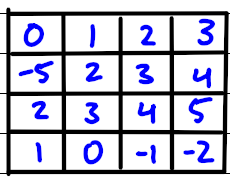
\includegraphics[width=0.25\textwidth]{q3_a.png}
        \end{figure}

        % \part Value function $ V_\pi \text{old}(s) = \E $
        \part Given a general MDP, rewards increase by $ r' = r + c $

        The value function is $ V_\pi \text{old}(s) $

        Then the new value function can be defined as: 

        \begin{align*}
            V_\pi \text{new}(s) &= \displaystyle\sum_{t = 0}^{\infty} \gamma^tr'(s_t) \\
            &= V_\pi \text{old}(s) + \displaystyle\sum_{t = 0}^{\infty} \gamma^tc
        \end{align*}
        where the old value function can be defined as $ V_\pi \text{old}(s) = \displaystyle\sum_{t = 0}^{\infty} \gamma^tr(s_t) $

        Since the horizon in infinite, then it becomes an infinite gemetric series as so:
        $$ \displaystyle\sum_{t = 0}^{\infty}\gamma^tc = \displaystyle\frac{c}{1 - \gamma}, \hspace*{10mm} \text{if} \mid \gamma \mid < 1 $$
        
        Thus, the new value function becomes:
        $$ V_\pi \text{new}(s) = V_\pi \text{old}(s) + \displaystyle\frac{c}{1 - \gamma} $$

        \part If we increase the value of $r_s$ to +2, and $ c = 3 $, then $ r_g = 5 + 3 = 8 $, and $ r_r = -2 $.

        Then the our new values become:

        \begin{figure}[H]
            \centering
            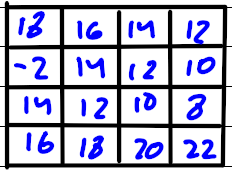
\includegraphics[width=0.25\textwidth]{q3_c.png}
        \end{figure}

        The above grid is only assuming that the agent follows the same optimal path from the first part. In reality, since the agent's reward is getting +2 for each non-terminal square, it would be more beneficial for the agent to take the longest path to the target square, as it would get more rewards. This could result in the agent getting stuck on squares 6, 7, 10 and 11 indefinitely as they would perpetually increase the agent's reward. 
    \end{parts}
\end{solution}

% \newpage
% \question[20]
% \input{q4.tex}

\end{questions}

\end{document}